% =============================================================================
\chapter{\textit{Data Storytelling}}\label{cap:storytelling}
% =============================================================================

A comunicação dos resultados foi pensada para quem decide na mesa de execução,
não para especialistas em estatística. Este capítulo descreve os princípios de
visualização adotados, a narrativa em três atos e a matriz de decisão que fecha o
projeto. A versão textual da narrativa está em \code{STORYTELLING.md}; a versão
visual, no notebook do \textit{Checkpoint}~3 e na primeira aba do painel.

\section{Princípios de visualização}\label{sec:principios}

Os gráficos seguem as recomendações de \citeonline{knaflic2018} de reduzir
elementos que não informam e direcionar a atenção para a mensagem. As regras
aplicadas em todos os gráficos do projeto foram:

\begin{alineas}
  \item \textbf{título-manchete}: o título principal de cada gráfico enuncia a
        conclusão (por exemplo, ``O fluxo explica o minuto em que acontece, mas
        quase nada do minuto seguinte''), e o subtítulo descreve o conteúdo;
  \item \textbf{cor com função fixa}: azul para compra ou série principal,
        laranja para venda ou alerta e tons de cinza para contexto, com paleta
        validada para daltonismo (protanopia, deuteranopia e tritanopia);
  \item \textbf{destaque seletivo}: apenas o que sustenta a conclusão recebe cor
        forte, como as três horas de maior volume na
        \autoref{fig:perfilhorario} ou o coeficiente do mesmo minuto na
        \autoref{fig:defasagens};
  \item \textbf{escalas honestas}: escala logarítmica para distribuições de
        cauda pesada, medianas quando a média distorce e faixa de ruído
        explícita nas correlações;
  \item \textbf{números no padrão brasileiro}: vírgula decimal, ponto como
        separador de milhar e horários em UTC com a conversão para BRT
        indicada.
\end{alineas}

\section{Narrativa em três atos}\label{sec:narrativa}

A narrativa ``Da calmaria ao estresse'' organiza os achados como uma história em
três atos, cada um ligado a uma pergunta de negócio e a uma decisão. A
\autoref{fig:storytelling} reúne as três evidências centrais em uma única
imagem, pensada para a apresentação executiva.

\begin{figure}[htbp]
\caption{\label{fig:storytelling}Síntese visual da narrativa ``Da calmaria ao estresse''}
\begin{center}
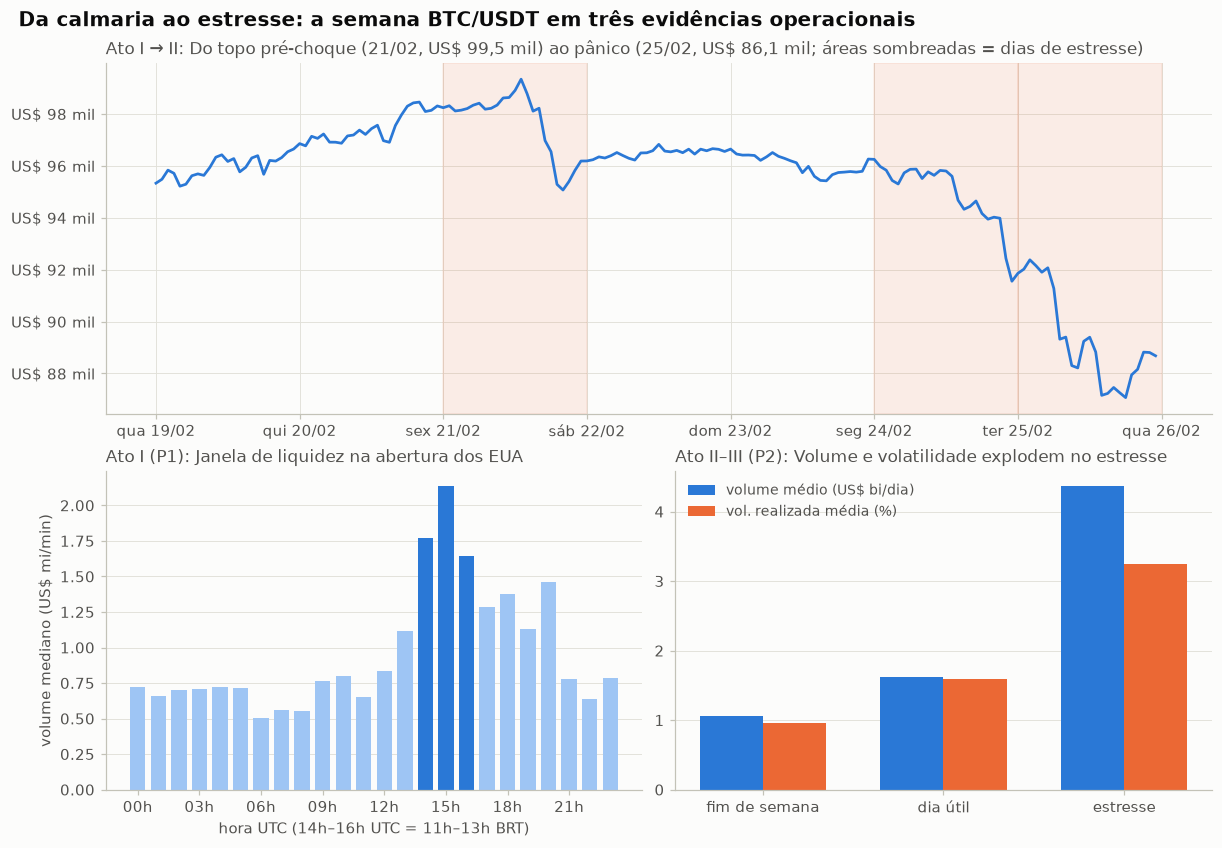
\includegraphics[width=\textwidth]{figuras/fig_storytelling.png}
\end{center}
\fontedados
\end{figure}

\textbf{Ato I -- O ritmo da calmaria (P1).} O mercado de BTC/USDT funciona
24 horas por dia, mas a liquidez não é uniforme: o volume mediano às 15h~UTC
(12h em Brasília) é 4,2 vezes o das 06h~UTC. O horário mais ativo coincide com a
abertura do mercado acionário americano. O dilema da mesa é que liquidez e
volatilidade caminham juntas ($\rho = 0,83$ entre as horas): entrar às 15h~UTC
reduz o impacto no livro, mas expõe uma ordem única a oscilações maiores.
\textbf{Decisão}: executar ordens institucionais dentro da janela líquida, sempre
fatiadas por TWAP ou VWAP.

\textbf{Ato II -- O choque e a escalada ao pânico (P2).} Na sexta-feira, 21/02, o
ataque à Bybit desencadeou uma mudança abrupta de regime. O bitcoin caiu 13,5\,\%
em quatro dias, com saldo vendedor em todos os dias da semana. Nos dias de
estresse, o volume foi 2,7 vezes e a volatilidade 2,0 vezes a de um dia útil; em
25/02 ocorreram 10,3 milhões de negócios e quase 10 mil ordens agressoras de
\usd~100 mil ou mais. Movimentos além de $3\sigma$ foram 6,9 vezes mais
frequentes que o previsto pela curva normal. \textbf{Decisão}: abandonar limites
estáticos e dimensionar a infraestrutura para picos de 4 a 5 vezes a carga
normal.

\textbf{Ato III -- Fluxo, modelos e os limites da eficiência (P3).} O fluxo
agressor empurra o preço no instante da execução (correlação de 0,388 no mesmo
minuto), mas quase não antecipa o minuto seguinte (0,022). Nenhum modelo
direcional, em 1 minuto ou 1 segundo, gerou ganho bruto capaz de pagar as taxas.
Em contrapartida, a volatilidade do próximo minuto é previsível fora da amostra
($R^2 = 0,385$). \textbf{Decisão}: usar a previsão de volatilidade para calibrar
limites e ritmo de execução, e não usar o OFI para operar direção.

\section{Matriz de decisão}\label{sec:matriz}

O \autoref{qua:matriz} consolida as recomendações em formato de matriz de
decisão, que é o fechamento da narrativa e o principal entregável para o
público executivo.

\begin{quadro}[htbp]
\caption{\label{qua:matriz}Matriz de decisão para a mesa de execução}
\begin{corpotabela}
\begin{tabularx}{\textwidth}{|L{2.7cm}|Y|L{5.4cm}|}
\hline
\textbf{Alavanca da mesa} & \textbf{Evidência empírica} & \textbf{Ação recomendada} \\ \hline
Janela de execução (TWAP/VWAP) & Pico às 15h~UTC com \usd~2,13 mi/min contra \usd~0,51 mi/min às 06h~UTC (4,2 vezes); Spearman entre volume e amplitude de 0,83 & Programar execuções grandes preferencialmente entre 14h e 16h~UTC (11h e 13h~BRT), sempre fatiadas; em dias de choque, monitorar deslocamentos da liquidez, como o pico às 07h~UTC de 25/02 \\ \hline
Limites de risco e \textit{slippage} & Em estresse, volatilidade realizada 2,0 vezes maior; 1,87\,\% dos minutos além de $3\sigma$ (6,9 vezes a normal); volatilidade de $t+1$ previsível ($R^2 = 0,385$; Spearman de 0,616) & Calibrar limites de \textit{slippage} e de perda dinamicamente pela volatilidade prevista pelo Ridge e pela realizada em janela móvel, abandonando bandas fixas baseadas na curva normal \\ \hline
Capacidade operacional & 25/02 teve 10,3 milhões de negócios (37\,\% da semana) e quase 10 mil ordens de \usd~100 mil ou mais (4,5 vezes um dia útil) & Dimensionar ingestão e roteamento para pelo menos 4 a 5 vezes o volume de negócios de um dia útil, sem perda de latência \\ \hline
Uso de sinais de fluxo (OFI) & Correlação de 0,388 no mesmo minuto e de 0,022 no minuto seguinte; ganho bruto direcional abaixo de 0,4~bps contra custos de 2 a 10~bps por perna & Não operar estratégia direcional com base no OFI; usá-lo apenas como filtro auxiliar para evitar cruzar o \textit{spread} contra um fluxo extremo imediato \\ \hline
\end{tabularx}
\end{corpotabela}
\fonteautores[Elaborado]
\end{quadro}

Os \textit{slides} da defesa final, último entregável pendente do
\textit{Checkpoint}~3, devem seguir esta mesma estrutura: problema, três atos e
matriz de decisão, reaproveitando as figuras deste documento.
